% !TEX program = xelatex
% !BIB program = bibtex
%%%%%%%%%%%%%%%%%%%%%%%%%%%%%%%%%%%%%%%%%%%%%%%%%%%%%%%
%%% LATEX FORMATTING - LEAVE AS IS %%%%%%%%%%%%%%%%%%%%
\documentclass[11pt]{article} % documenttype: article
\usepackage[top=20mm,left=20mm,right=20mm,bottom=15mm,headsep=15pt,footskip=15pt,a4paper]{geometry} % customize margins
\usepackage{times} % fonttype
\usepackage{csquotes}
\usepackage{xeCJK}
\usepackage{graphicx}
\usepackage[backend=bibtex, sorting=none]{biblatex}

\addbibresource{shifei_chen_assignment_2.bib}
\graphicspath{ {./images/} }

\makeatletter         
\def\@maketitle{   % custom maketitle 
\begin{center}
{\bfseries \@title}
{\bfseries \@author}
\end{center}
\smallskip \hrule \bigskip }

%%%%%%%%%%%%%%%%%%%%%%%%%%%%%%%%%%%%%%%%%%%%%%%%%%%%%%%%%%%%%%%%%%%%
%%% MAKE CHANGES HERE %%%%%%%%%%%%%%%%%%%%%%%%%%%%%%%%%%%%%%%%%%%%%%
\title{{\LARGE Natural Language Processing: Assignment 2}\\[1.5mm]} % Replace 'X' by number of Assignment
\author{Shifei Chen} % Replace 'Firstname Lastname' by your name.

%%%%%%%%%%%%%%%%%%%%%%%%%%%%%%%%%%%%%%%%%%%%%%%%%%%%%%%%%%%%%%%%%%%%
%%% BEGIN DOCUMENT %%%%%%%%%%%%%%%%%%%%%%%%%%%%%%%%%%%%%%%%%%%%%%%%%
%%% From here on, edit document. Use sections, subsections, etc.
%%% to structure your answers.
\begin{document}
\maketitle

\section{POS-Tagging}

My tagger achieved an accuracy of 93.10\% by using parameters \texttt{-t 3 -f 5 -s 5}. Here are some examples of errors my tagger made.

\begin{displayquote}
  1. "From the AP comes this story."
\end{displayquote}

"AP" was mistagged as a NOUN rather than a PRON. This is pretty obvious since AP indeed is the name of the news agency.

\begin{displayquote}
  2. "The sheikh in wheel-chair has been attacked with a F-16-launched bomb."
\end{displayquote}

"F" was tagged as a NOUN in the gold standard and a PRON in my result. I think both of the tags are not correct. Here "F-16-launched" should be treated as a single adjective. If we have to separate them, I would believe that "F" is a pronoun as it is a part of the model name of a plane.

\begin{displayquote}
  3. "US troops there clashed with guerrillas in a fight that left one Iraqi dead."
\end{displayquote}

My tagger believed the word "Iraqi" is a ADJ rather than a PRON. A English speaker shouldn't make that mistake since he can see clearly that the clause "left one Iraqi dead" is the consequnce of the fight and because of that, "left" is a verb and "dead" is an adjective. My tagger might not be able to trace that far away. It might simply looked at the words around "Iraqi" and believed this fit the structure of num. + adj. + noun.

\begin{displayquote}
  4. "Xinhua alleged that 'Many of the Iraqis, who suffer ...'"
\end{displayquote}

"that" should be a SCONJ instead of a DET because of the word "alleged" and the fact that everything after "that", from a semantic prospective, is the content of Xinhua agency's allegation.

\begin{displayquote}
  5. "2015 is going to rock!"
\end{displayquote}
We know "rock" can be a noun or a verb but in this sentence, a verb will make more sense semantically. Hence the word "to" should be a particle than a preposition.

In general, I think in my tagger only part of the mistakes are considered to be genuinely ambiguous, for example ADP vs. PART. There are still plenty of cases which are not ambiguous to human beings at all. The tagger is restricted to look forward or backward only $N$ words (specified by the parameter \texttt{-t}) therefore it cannot have a better understanding of the context overall, especially in sentences consist of clauses. Another issue is the lack of semantics analysis. It made my tagger confused. There is a sentence in our corpus goes
\begin{displayquote}
  ... they hear a company who's stated goals include "Don't be evil," ...
\end{displayquote}

My tagger tagged "evil" as a noun while our golden standard marked it as an adjective. Both of them make sense, although personally I believe that company is Google hence I would choose ADJ. Senteces like "I'm going to work.", "to" being a particle or preposition makes sense in either way since "work" can mean the action (verb) or the place (pronoun/noun). These two problems exist in our golden standard as well.
\begin{displayquote}
  ... the price would be too high for investors to make a real profit.
\end{displayquote}
In this sentence "for" should be a prepostion, not a subordinating conjuction. There is no clause in this sentence.

I found several tagsets for my mother language, Chinese: the Chinese Penn Treebank POS tagset\cite{xia2000part}, an SVMTool-Based Chinese POS Tagger\cite{王丽杰2009基于}, FudanNLP\cite{qiu2013fudannlp}, etc. Here we take a closer look at the Chinese Penn Treebank tagset. Comparing to its English siblings, the Chinese tagset has 33 tags. Words ``把" and ``被", which means "make sth. to do" and passive voice, respectfully, are separated from other verbs and prepostions since their identities are still highly controversial. Another intresting thing I have noticed is that ``的", ``地" and ``得", which are the three most common particles, are categorised into DEC, DEG, DER and DEV. This is a reasonable choice as their appearence usually gives people hints about the part-of-speech of words around them, like ``得" usually indicates the word it follows is always a verb and the word after it is usually an adverb.

Therefore I hold the idea that tokenization doesn't necessarily has to be done before tagging in some languages like Chinese, though most tagging algorithms assume that a process of tokenization has been applied to the tags\cite[157]{JurafskyMartin200805}. Of course tagging could benefit from tokenization because it gives information of word boundaries, sentence boundaries, average word length, etc. On the other hand, tagging could also help improve tokenization as different part-of-speeches will have impacts on tokenizaiton. For example distinguishing "." as a punctuation from a symbol of abbreviation. Another example is like in languages like Japanese, its particles usually contains rich information about the structure and semantics. ``好きだ" ``だ" at the end of the sentence usually means it is an auxiliary verb and we can therefore separate it from the other parts of the sentence. It also tell us that ``好き" here should be a noun or a na-adjective (It actually means "like" and in Japanese "like" is an adjective). Tagging does not need to be after tokenization and I believe it is better if they can be carried out simultaneously.

Finally in Lab 6 we did an invesitigation on key sequences and predicted words in mobile phone inputs. By definition HMM models should always have a sequence of $T$ observations (or signals) $O_1, O_2, O_3, ..., Q_T$, and a set of $N$ states $Q_1, Q_2, Q_3, ..., Q_N$\cite[177]{JurafskyMartin200805}. If we observe the sequences of number keys then our states will be letters of the words because this is what we see at the surface. Our signals will be the numbers as they are not what we can directly observe and they are hidden behind the predicted words. On the other hand, when we apply HMM models to POS tagging, what we see is a sequence of words and what we need to find out is the sequence of tags corrsponding to them. Words are the signals and tags are the hidden states.

\section{Lemmatisation}

\subsection{Lemmatizer Analysis}
After tunning my lemmatizer to achieve a score of 94.71\%, here are five of the remainning issues.

1. Irregular Nouns/Verbs

Some nouns and verbs do not follow the inflection rules and since they don't follow any rules I have to use the method of exhaustion to tackle them. I have built a dict in my lemmatizer but it is still far from compelete. And as the lab instruction had pointed out, the lexicon could only grow in a more sophisticated lemmatizer.

2. Overlemmatisation

Some words look very much like they are already in a inflection form but actually they are not. For example "bring" was mistook by my lemmatizer to believe it is in its progressive form. Again a comprehesive lexicon will help us solve this problem. But it could also be beneficial if we provide more information by tagging different forms of verbs/nouns with different tags, like VB/VBG/VBD in the Penn Treebank tagset.

3. Constant Doubling

For words like "cut", "big" we have to repeat the final constant and then make any conjugation. The general rule is a single vowel surrounded by two constants and it should exist in any modern lemmatizers.

4. Different Meanings with Singluar and Plural Form

The meaning of some nouns can change slightly with their singular and plural form, e.g. "troop" means a small group of soilders while "troops" usually means the army in general. In Lemmatisation it is hard to tell the difference bewteen these two words as we usually work with a single word at a time. We lack the context to judge its semantic. One possbile solution I can think of is that we can mark their with different tags, e.g. NN and NNS, just like the overlemmatisation problem.

5. The Hidden "e"

The is the most common problem in my lemmatizer and it relates to pronounciation as well. The "e" in words like "take" changes the pronounciation of the vowel "a" hence it is necessary to be restored during lemmatisation. But when I was thinking how to program the rules to restore it I found that it is exactly the same rule to deal with a closed heavy syllable at the end of the word--a vowel surrounded by two constants. The hidden "e" case usually happenes in longer words (more than 4 letters) and we can use that feature to distinguish them besides a big lexicon.

\subsection{FST Diagram}

My FST diagram goes as the picture below.

\begin{figure}[h]
  \centering
  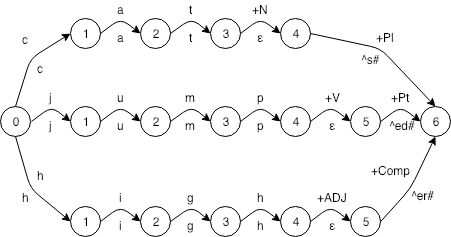
\includegraphics[width=0.5\textwidth]{images/figure_fst.png}
  \caption{FST for "cats", "jumped" and "higher"}
\end{figure}

We have three words "cats", "jumped" and "higher" on the surface level. Their stems are "cat", "jump" and "high", respectfully. We also need to know their lexical level to draw this diagram. For example for "jumped" it is "jump +V +Pt(Past tense)". Then just expand the Fig 3.13 on the textbook\cite[61]{JurafskyMartin200805} with some necessary changes to fit both verbs and adjectives and I got the diagram above.

\subsection{Tagging in Morphologically Rich Languages}

English is not a morphologically rich language, therefore it has two advantages compared with other highly inflectional languages like Finnish. First each word's role in the sentence is much less, which means it usually carries fewer tags than the one in morphologically rich languages. As a result we can see that English tagsets have way less tags\cite[162]{JurafskyMartin200805}. Another issus is that, during tagging process different inflections of the same stem will be treated as different words, hence highly inflectional languages will have a higher precentage of unknow words. If we recall that an HMM tagging algorithm using trigram tags will often has problems with data sparsity\cite[149]{JurafskyMartin200805}, then here we will be in a deeper trouble as we now have not only unseen tag combinations in our test set but also way more unseen words. Moreover as modern taggers tend to give as many morphological tags as possbile and treat them as a single complex tag when tagging a morphologically rich language, there might be problems with unseen tag combinations too. We need good interpolation algorithms to solve this problem.

\printbibliography

\end{document}
